\begin{center}
  \Large
  \textbf{BIOGRAFI PENULIS}
\end{center}

\addcontentsline{toc}{chapter}{BIOGRAFI PENULIS}

\vspace{2ex}

\begin{wrapfigure}{L}{0.3\textwidth}
  \centering
  \vspace{-3ex}
  % Ubah file gambar berikut dengan file foto dari mahasiswa
  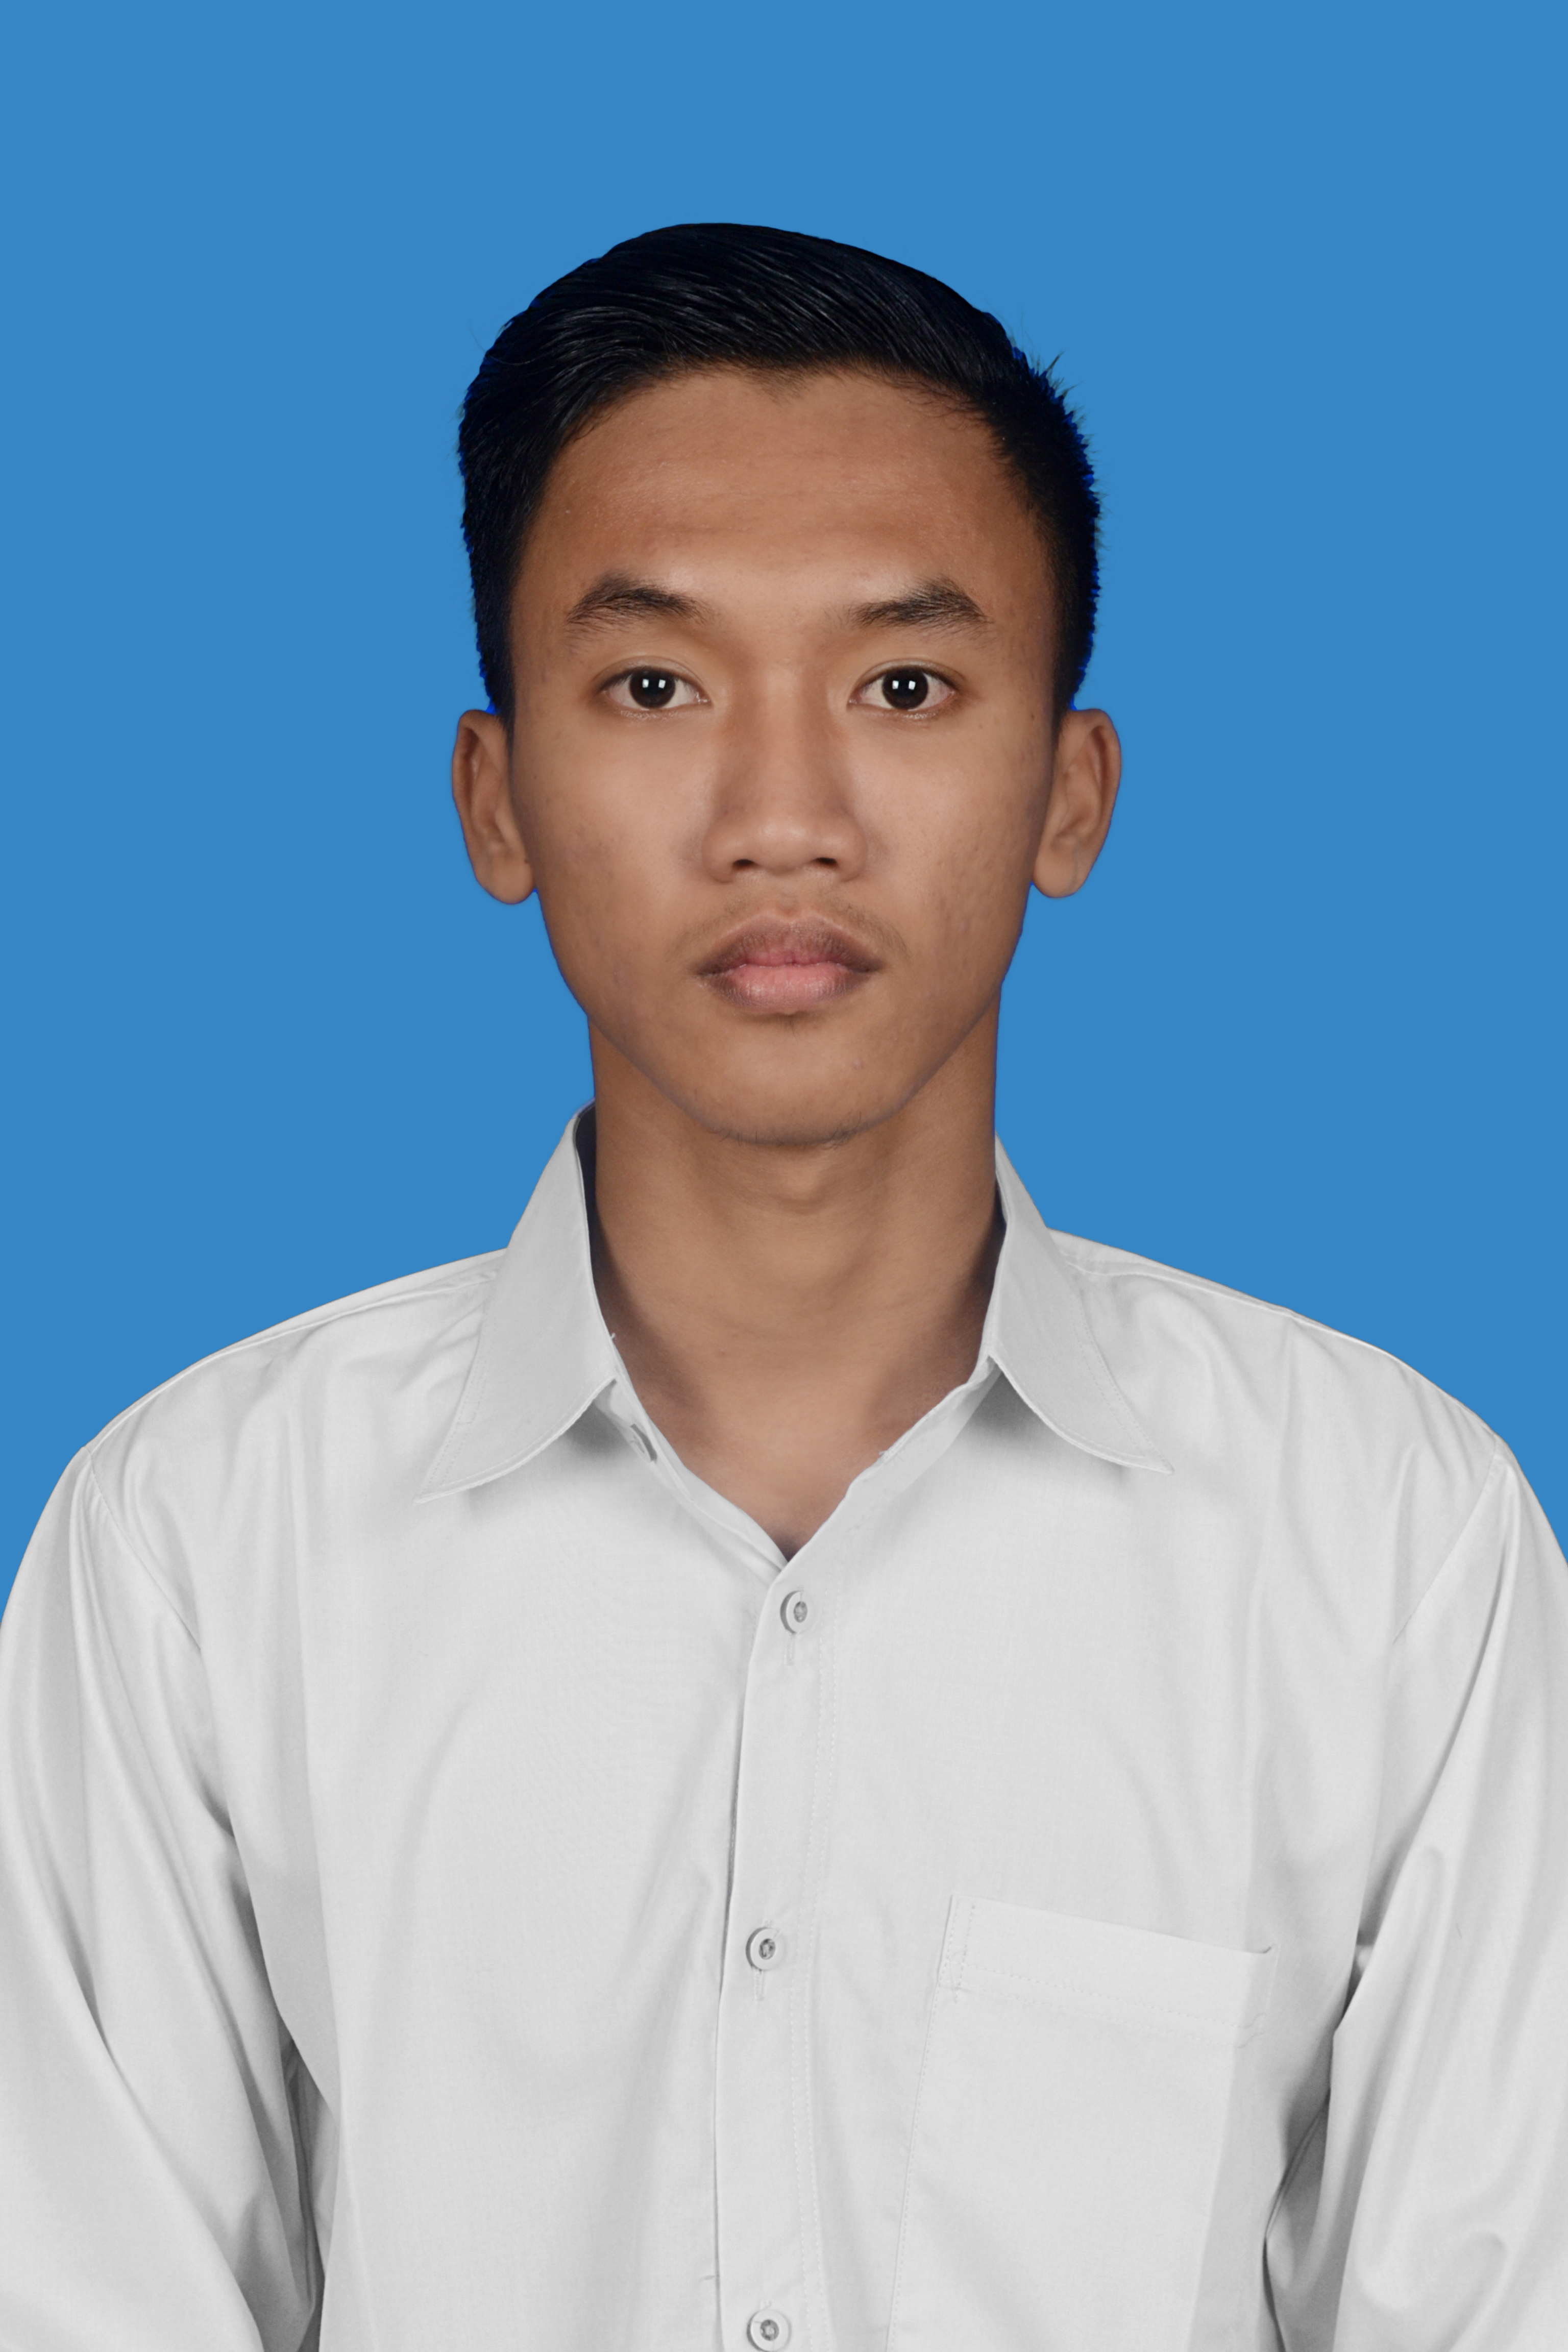
\includegraphics[width=0.3\textwidth]{gambar/dhani.png}
  \vspace{-4ex}
\end{wrapfigure}

% Ubah kalimat berikut dengan biografi dari mahasiswa
\name{}, lahir pada \linebreak tanggal 1 Desember 2000, Trenggalek. Merupakan seseorang \linebreak mahasiswa yang berasal dari Institut Teknologi
Sepuluh \linebreak Nopember departemen Teknik Komputer. Penulis merupakan anak pertama dari 2 bersaudara. 
Penulis telah menempuh \linebreak pendidikan formal yaitu di TKIT Mutiara Ummat Trenggalek, sdit Mutiara Ummat Trenggalek, MTsN 1 Trenggalek dan MAN 2 Tulungagung.
Setelah lulus dari MAN 2 Tulungagung tahun 2019, Penulis mengikuti SNMPTN dan diterima di Departemen Teknik Komputer FTEIC - ITS pada tahun 2019 dan terdaftar dengan NRP 07211940000016.
Dalam masa kuliah, penulis tertarik pada bidang Mobile Development dan IoT. Selain itu, penulis juga aktif dalam organisasi Himpunan Mahasiswa \linebreak Departemen Teknik Komputer ITS selama kurang 2 tahun.
Penulis juga aktif mengikuti kegiatan Kampus Merdeka, yaitu Studi Independen Bersertifikat pada program Bangkit Academy 2022 by Google, GoTo, Traveloka - Android Learning Path.
